%!TEX root =  main.tex
\chapter*{Chapter 5 Concentration of Measure}
\label{sec:5}

\noindent\textbf{5.1}
(\textsc{Variance of average})
Let $X_{1}, X_{2}, \ldots, X_{n}$ be a sequence of independent and identically distributed random variables with mean $\mu$ and variance $\sigma^{2}<\infty$.
Let $\hat{\mu}=\frac{1}{n} \sum_{t=1}^{n} X_{t}$ and show that $\mathbb{V}[\hat{\mu}]=\mathbb{E}\left[(\hat{\mu}-\mu)^{2}\right]=\sigma^{2} / n$.

\begin{proof}
	We start straight from the definition:

	\begin{equation*}
		\begin{aligned}
		&\mathbb{V}[\hat{\mu}]\\
		= &\mathbb{E}((\hat{\mu }-\mu)^2)\\
		= &\mathbb{E}((\frac{1}{n}\sum_{t=1}^{n}{X_t}-\mu)^2)\\
		= &\mathbb{E}(\frac{1}{n^2}\sum_{t=1}^{n}{(X_t - \mu)^2})\\
		= &\frac{1}{n^2}\sum_{t=1}^{n}{\mathbb{E}(X_t - \mu)^2}\\
		= &\frac{1}{n^2}\sum_{t=1}^{n}{\sigma^2}\\
		= &\frac{\sigma^2}{n}
		\end{aligned}
	\end{equation*}			

\end{proof}

\noindent\textbf{5.2}
% From the definition of expectation:
% $$
% {\displaystyle \operatorname {E} (X)=\int _{-\infty }^{\infty }xf(x)\,dx}{\displaystyle \operatorname {E} (X)=\int _{-\infty }^{\infty }xf(x)\,dx}$$
% \newline

% \noindent
% However, X is a non-negative random variable thus,
% $$
% {\displaystyle \operatorname {E} (X)=\int _{-\infty }^{\infty }xf(x)\,dx=\int _{0}^{\infty }xf(x)\,dx}{\displaystyle \operatorname {E} (X)=\int _{-\infty }^{\infty }xf(x)\,dx=\int _{0}^{\infty }xf(x)\,dx}$$
% \newline

% \noindent
% From this we can derive,
% \begin{align*}
%     {\displaystyle \operatorname {E} (X)&=\int _{0}^{a}xf(x)\,dx+\int _{a}^{\infty }xf(x)\,dx\geq \int _{a}^{\infty }xf(x)\,dx\geq \int _{a}^{\infty }af(x)\,dx\\
%     &=a\int _{a}^{\infty }f(x)\,dx=a\operatorname {Pr} (X\geq a)}{\displaystyle \operatorname {E} (X)=\int _{0}^{a}xf(x)\,dx+\int _{a}^{\infty }xf(x)\,dx\\
%     &\geq \int _{a}^{\infty }xf(x)\,dx\geq \int _{a}^{\infty }af(x)\,dx\\
%  &=a\int _{a}^{\infty }f(x)\,dx=a\operatorname {Pr} (X\geq a)}
% \end{align*}

% From here, dividing through by a allows us to see that
% $$
% {\displaystyle \Pr(X\geq a)\leq \operatorname {E} (X)/a}{\displaystyle \Pr(X\geq a)\leq \operatorname {E} (X)/a}
% $$







\noindent\textbf{5.3} Compare the Gaussian tail probability bound on the right-hand side of $(5.4)$ and the one on (5.2). What values of $\varepsilon$ make one smaller than the other? Discuss your findings.

\begin{proof}
	Two-slided tail directly in terms of the variance in (5.2) is $\mathbb{P}(|\hat{\mu}-\mu| \geq \varepsilon) \leq \frac{\sigma^{2}}{n \varepsilon^{2}}$. And in (5.4) 
	\begin{equation}
	\begin{aligned}
 	\notag
	\mathbb{P}(\hat{\mu} \geq \mu+\varepsilon) &=\mathbb{P}\left(S_{n} / \sqrt{\sigma^{2} n} \geq \varepsilon \sqrt{n / \sigma^{2}}\right) \approx \mathbb{P}\left(Z \geq \varepsilon \sqrt{n / \sigma^{2}}\right) \\
	& \leq \sqrt{\frac{\sigma^{2}}{2 \pi n \varepsilon^{2}}} \exp \left(-\frac{n \varepsilon^{2}}{2 \sigma^{2}}\right)
	\end{aligned}
	\end{equation}

	We need to compare $\frac {\sigma^2} {2 n \varepsilon^2}$ and $ \sqrt{\frac{\sigma^{2}}{2 \pi n \varepsilon^{2}}} \exp \left(-\frac{n \varepsilon^{2}}{2 \sigma^{2}}\right)$ and we can define:

	\begin{equation}
	\begin{aligned}
		 \notag
		f(\varepsilon) = \frac {\sigma^2} {2 n \varepsilon^2}- \sqrt{\frac{\sigma^{2}}{2 \pi n \varepsilon^{2}}} \exp \left(-\frac{n \varepsilon^{2}}{2 \sigma^{2}}\right)
	\end{aligned}	
	\end{equation}


	Let $x = \frac {\sigma ^2} {2 n \varepsilon^2}$, then 

	\begin{equation}
	\begin{aligned}
		 \notag
		f(x) = x - \frac {\sqrt {x}} {\sqrt{\pi}} \exp(\frac 1 {4 x})
	\end{aligned}
	\end{equation}


	When $f(x) = 0$, the Lambert form of the equation could be writen as:

	\begin{equation}
	\begin{aligned}
 	\notag
	\frac 1 \pi = x \exp(- \frac {1} {2x})
	\end{aligned}	
	\end{equation}

	with the $\frac 1 {2x} = u$, the equation is transformed into
	
	\begin{equation}
	\begin{aligned}
	\notag
	u \exp(u) = \frac {\pi} {2}
	\end{aligned}	
	\end{equation}

	Solve the equation, $u = W_0(\frac \pi 2)$, and then $f(x) = 0$ when

	\begin{equation}
	\begin{aligned}
	\notag
\varepsilon = \sqrt{\frac {W_0(\frac {\pi} {2}) \sigma^2} {n}}
	\end{aligned}	
	\end{equation}

	In order to judge the positive or negative of the $f(x)$, we need to judge the monotonicity in addition to solving the zero point. $f'(x) = x - \frac {\sqrt x}{\pi} exp(\frac 1 {4x})$, and from the picture, $f'(x)$ is always bigger than 0. Thus, when $\varepsilon > \sqrt{\frac {W_0(\frac {\pi} {2}) \sigma^2} {n}}$, (5.2) is greater than (5.4), otherwise (5.2) is smaller.


\end{proof}




\noindent\textbf{5.4} Let $X$ be a random variable on $\RR$ with density with respect to the Lebesgue measure of $p(x)= \abs{x}\exp\bracket{-x^2/2}/2$. Show the following:
\begin{enumerate}
	\item[(a)] $\PP{\abs{X}\ge \varepsilon} = \exp(-\varepsilon^2/2)$
	\item[(b)] $X$ is not $\sqrt{2-\varepsilon}$-subgaussian for any $\varepsilon>0$.
\end{enumerate}

\begin{proof}
\begin{enumerate}
	\item[(a)] 
	\begin{align*}
		\PP{\abs{X}\ge \varepsilon} &=\int^{-\varepsilon}_{-\infty} 
		\frac{\abs{x}}{2}\exp\bracket{-x^2/2} d x +  \int_{\varepsilon}^{+\infty} \frac{\abs{x}}{2} \exp\bracket{-x^2/2} d x \\
		&=\int^{-\varepsilon}_{-\infty} -\frac{x}{2} \exp\bracket{-x^2/2}/2 d x +  \int_{\varepsilon}^\infty \frac{x}{2} \exp\bracket{-x^2/2} d x \\
		&= \int_{\varepsilon}^\infty x \exp\bracket{-x^2/2} d x \\
		&= \exp\bracket{-\varepsilon^2/2}\,.
	\end{align*}
	\item[(b)] 
	According to the definition of the sub-gaussian random variables, to prove $X$ is not $\sqrt{2-\varepsilon}$-subgaussian, we want to prove $\exists \lambda \in \RR$ such that 
	\begin{align*}
		\EE{\exp\bracket{\lambda X}} \le \exp\bracket{\frac{\lambda^2 (2-\varepsilon)}{2}} \triangleq g(\lambda) \,.
	\end{align*}
	For the LHS, there is
	\begin{align*}
		\EE{\exp\bracket{\lambda X}} &= 	\int_{-\infty}^{+\infty} \exp(\lambda x) \frac{|x|}{2} \exp(-x^2/2) dx \\
		&= \frac{1}{2}\exp(\lambda^2/2)\int_{-\infty}^{+\infty} \abs{t+\lambda} \exp(-t^2/2)dt \\
		&= \frac{\exp(\frac{\lambda^2}{2})}{2} \bracket{\int_{-\infty}^{-\lambda} (-t-\lambda) \exp(-t^2/2)dt+\int_{-\lambda}^{+\lambda} (t+\lambda) \exp(-t^2/2)dt + \int_{\lambda}^{+\infty}(t+\lambda) \exp(-t^2/2)dt} \\
		&= \frac{\exp(\frac{\lambda^2}{2})}{2} \bracket{{2\exp(-\frac{\lambda^2}{2})} + 2\lambda \int_0^\lambda \exp(-t^2/2)dt } \\
		&= 1 + \lambda \exp(\frac{\lambda^2}{2})\int_{0}^{\lambda} \exp(-t^2/2) dt \triangleq f(\lambda) \,,.
	\end{align*}
	Define $F(\lambda) = f(\lambda) - g(\lambda)$, now we want to prove $\exists \lambda \in \RR, F(\lambda)>0$. By computation, we found that $F(0)=0, F'(0) = 0, F''(0)=\varepsilon >0$. We can then conclude that $(0,0)$ is a minima of $F$, thus $\exists \delta>0, \forall \lambda\in (-\delta,\delta), F(\lambda)>0$. We then get the desired result. 
\end{enumerate}
\end{proof}



% (a)
% \begin{equation}
% P(|X|\geq \varepsilon) = P(X\geq\varepsilon)I\{X\geq 0\}+P(X\leq -\varepsilon)I\{X< 0\}
% =\int_{\varepsilon}^{\infty} \frac{x}{2} exp\{ \frac{-x^2}{2}\} dx + \int_{-\infty}^{\varepsilon} \frac{-x}{2} exp\{ \frac{-x^2}{2}\} dx
% \end{equation}

% Calculate the above formula and get the result ,

% $P(|X|\geq \varepsilon) =\frac{1}{2} exp\{ \frac{-\varepsilon^2}{2}\} + \frac{1}{2} exp\{ \frac{-\varepsilon^2}{2}\}$

% $=exp\{ \frac{-\varepsilon^2}{2}\}$


% (b)

% Let's start with a lemma:

% If X is $\sigma-$subgaussian,then $P(|X|>t) \leq exp\{ -b \varepsilon^2\}$ , where $b=exp\{ -\sigma^2\}$

% The proof of lemma is omitted.

% It can be seen from the first question , $P(|X|\geq \varepsilon) = exp\{ \frac{-\varepsilon^2}{2}\}$

% The comparison of the two formulas shows that , $0<b\leq 1/2$ . That is, $\sigma\geq \sqrt{ln2}$

% By topic condition , $\sigma = \sqrt{2-\varepsilon}$

% Hence , $\varepsilon \leq 2-ln2$ , this is in contradiction with the arbitrariness of $\varepsilon$

\noindent\textbf{5.5}
\textsc{(Berry–Esseen inequality)} Let $X_1,X_2,\cdots,X_n$ be a sequence of independent and identically distributed random variables with mean $\mu$, variance $\sigma^2$ and bounded third absolute moment:
\begin{align*}
    \rho=\mathbb{E}[|X_1-\mu|^3]<\infty
\end{align*}
Let $S_n=\sum^n_{t=1}(X_t-\mu)/\sigma$. The Berry–Esseen theorem shows that
\begin{align*}
    \sup_x\left|\mathbb{P}\left(\frac{Sn}{\sqrt{n}}\leq x \right)-\underbrace{\frac{1}{\sqrt{2\pi}}\int^x_{-\infty}\exp(-y^2/2)dy}_{\Phi(x)} \right|\leq\frac{C\rho}{\sqrt{n}}\,,
\end{align*}
where $C<1/2$ is a universal constant.
\begin{enumerate}
	\item[(a)] Let $\hat{\mu}_n=\frac{1}{n}\sum^n_{t=1}X_t$ and derive a tail bound from the Berry–Esseen theorem. That is, give a bound of the form $\mathbb{P}(\hat{\mu}_n\geq\mu+\epsilon)$ for positive values of $\epsilon$.
	\item[(b)] Compare your bound with the one that can be obtained from the Cram{\'e}r–Chernoff method. Argue pro- and contra- for the superiority of one over the other.
\end{enumerate}

\begin{proof}
\begin{enumerate}
	\item[(a)] 
	\begin{align}\label{eq:Ex5.5_BEIneq}
	    \mathbb{P}(\hat{\mu}_n\geq \mu+\epsilon)&=\mathbb{P}\left(\frac{1}{n}\sum^n_{t=1}(X_t-\mu)\geq\epsilon\right)\notag\\
	    &=\mathbb{P}\left(\frac{\sum^n_{t=1}(X_t-\mu)}{\sqrt{n}\sigma}\geq\frac{\epsilon\sqrt{n}}{\sigma}\right)\notag\\
	    &=1-\mathbb{P}\left(\frac{\sum^n_{t=1}(X_t-\mu)}{\sqrt{n}\sigma}\leq\frac{\epsilon\sqrt{n}}{\sigma}\right)\notag\\
	    &\leq 1-\Phi\left(\frac{\epsilon\sqrt{n}}{\sigma}\right)+\frac{C\rho}{\sqrt{n}}\notag\\
	    &=\mathbb{P}\left(Z>\frac{\epsilon\sqrt{n}}{\sigma}\right)+\frac{C\rho}{\sqrt{n}}\quad\text{where}\quad Z\sim\mathcal{N}(0,1)\notag\\
	    &\leq\sqrt{\frac{\sigma^2}{2\pi n\epsilon^2}}\exp\left(-\frac{n\epsilon^2}{2\sigma^2}\right)+\frac{C\rho}{\sqrt{n}}\,.
	\end{align}
	\item[(b)] We further assume that $X_t$ is $\sigma$-subgaussian for all $t\in[n]$. Applying Cram{\'e}r–Chernoff method shows that
	\begin{align}\label{eq:Ex5.5_CCEneq}
	    \mathbb{P}(\hat{\mu}-\mu>\epsilon)\leq\exp\left(-\frac{n\epsilon^2}{2\sigma^2}\right)\,.
	\end{align}
	We now discuss the pros and cons based on the additional multiplicative term $\sqrt{\frac{\sigma^2}{2\pi n\epsilon^2}}$ and the additive term $\frac{C\rho}{\sqrt{n}}$ in Eq.\eqref{eq:Ex5.5_BEIneq}. When $n$ is large enough, the terms $\sqrt{\frac{\sigma^2}{2\pi n\epsilon^2}}$ and $\frac{C\rho}{\sqrt{n}}$ will both be small. It follows that Eq.\eqref{eq:Ex5.5_BEIneq} will be tighter when $n\rightarrow \infty$ but will be looser when $n$ is small than Eq.\eqref{eq:Ex5.5_CCEneq}.
\end{enumerate}
\end{proof}


\noindent\textbf{5.6} (CENTRAL LIMIT THEOREM) We mentioned that invoking the CLT to approximate the distribution of sums of independent Bernoulli random variables using a Gaussian can be a bad idea. Let $X_{1}, \ldots, X_{n} \sim \mathcal{B}(p)$ be independent Bernoulli random variables with common mean $p=p_{n}=\lambda / n$, where $\lambda \in(0,1)$. For $x \in \mathbb{N}$ natural number, let $P_{n}(x)=\mathbb{P}\left(X_{1}+\cdots+X_{n}=x\right)$.
\begin{enumerate}
	\item [(a)] Show that $\lim _{n \rightarrow \infty} P_{n}(x)=e^{-\lambda} \lambda^{x} /(x !)$, which is a Poisson distribution with parameter $\lambda$.
	\item [(b)] Explain why this does not contradict the CLT, and discuss the implications of the Berry-Esseen.
	\item [(c)] In what way does this show that the CLT is indeed a poor approximation in some cases?
	\item [(d)] Based on Monte Carlo simulations, plot the distribution of $X_{1}+\cdots+X_{n}$ for $n=30$ and some well-chosen values of $\lambda$. Compare the distribution to what you would get from the CLT. What can you conclude?
\end{enumerate}

\begin{proof}
	

\begin{figure}[tbh!]
		\centering
		\subfigure[$\lambda=0.1$]{
		\begin{minipage}[t]{0.25\linewidth}
		\centering
		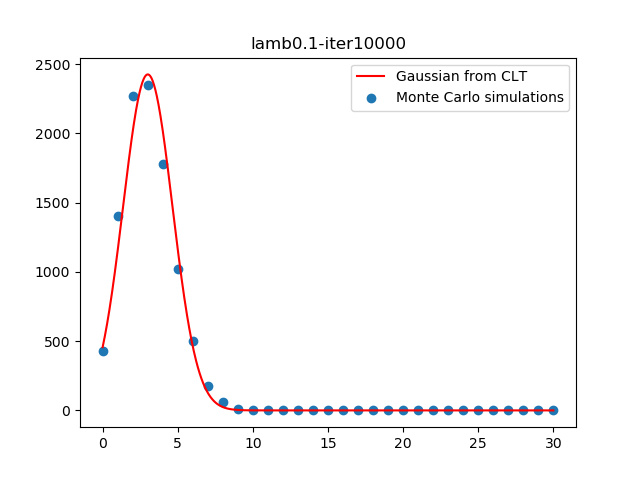
\includegraphics[width=4cm]{5_6_picture/lamb0_1-iter10000.png}
		%\caption{fig1}
		\end{minipage}%
		}%
		\subfigure[$\lambda=0.2$]{
		\begin{minipage}[t]{0.25\linewidth}
		\centering
		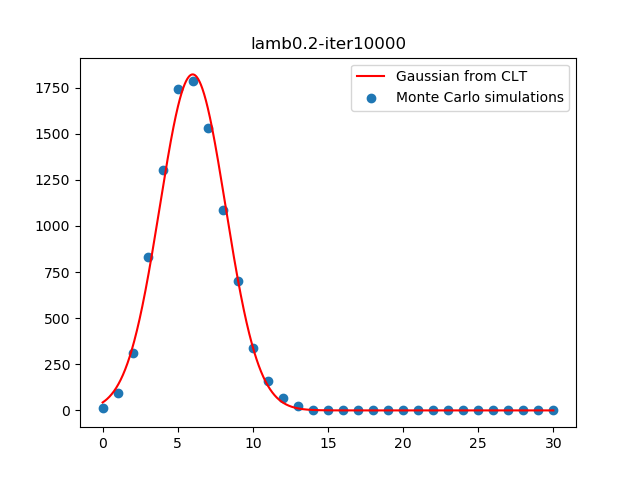
\includegraphics[width=4cm]{5_6_picture/lamb0_2-iter10000.png}
		%\caption{fig2}
		\end{minipage}%
		}%
		\subfigure[$\lambda=0.3$]{
		\begin{minipage}[t]{0.25\linewidth}
		\centering
		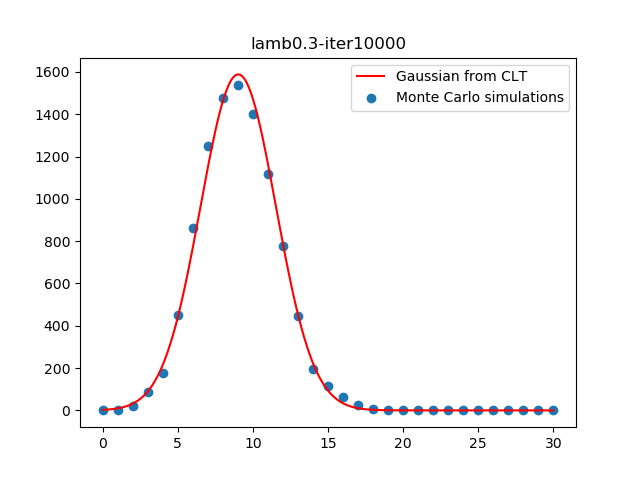
\includegraphics[width=4cm]{5_6_picture/lamb0_3-iter10000.png}
		%\caption{fig2}
		\end{minipage}%
		}%

		\subfigure[$\lambda=0.4$]{
		\begin{minipage}[t]{0.25\linewidth}
		\centering
		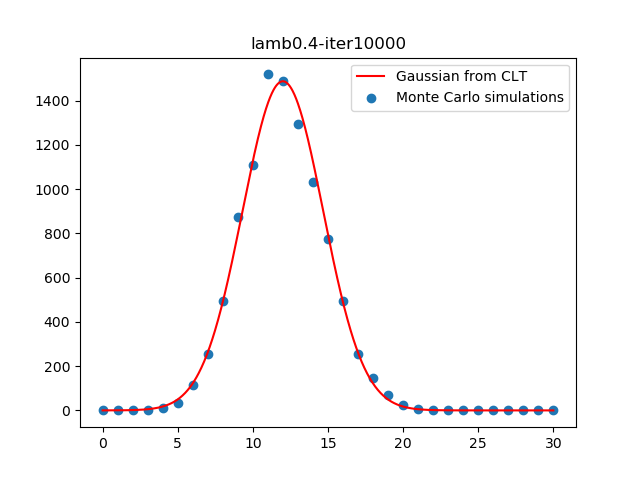
\includegraphics[width=4cm]{5_6_picture/lamb0_4-iter10000.png}
		%\caption{fig2}
		\end{minipage}
		}%
		\subfigure[$\lambda=0.5$]{
		\begin{minipage}[t]{0.25\linewidth}
		\centering
		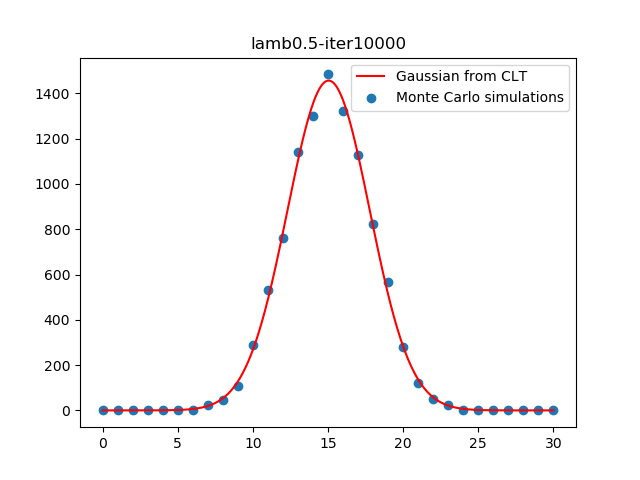
\includegraphics[width=4cm]{5_6_picture/lamb0_5-iter10000.png}
		%\caption{fig2}
		\end{minipage}
		}%
		\subfigure[$\lambda=0.6$]{
		\begin{minipage}[t]{0.25\linewidth}
		\centering
		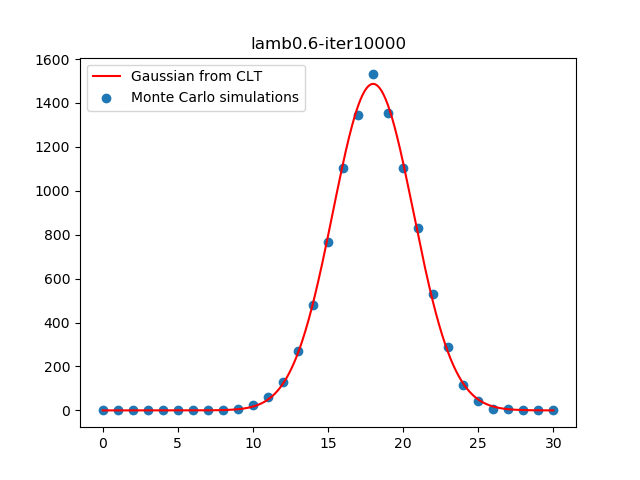
\includegraphics[width=4cm]{5_6_picture/lamb0_6-iter10000.png}
		%\caption{fig2}
		\end{minipage}%
		}%


		\subfigure[$\lambda=0.7$]{
		\begin{minipage}[t]{0.25\linewidth}
		\centering
		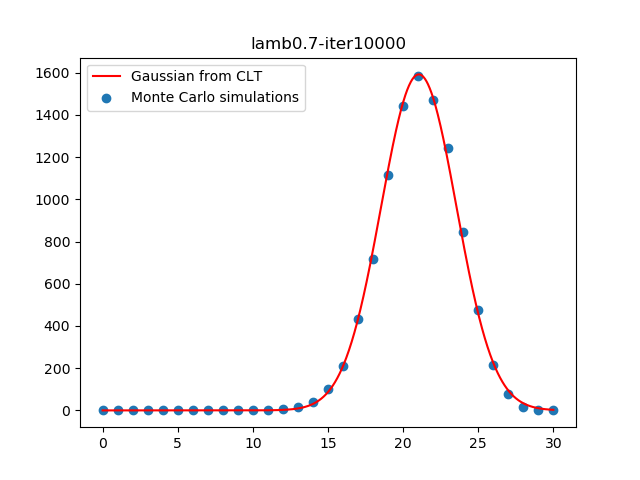
\includegraphics[width=4cm]{5_6_picture/lamb0_7-iter10000.png}
		%\caption{fig2}
		\end{minipage}%
		}%
		\subfigure[$\lambda=0.8$]{
		\begin{minipage}[t]{0.25\linewidth}
		\centering
		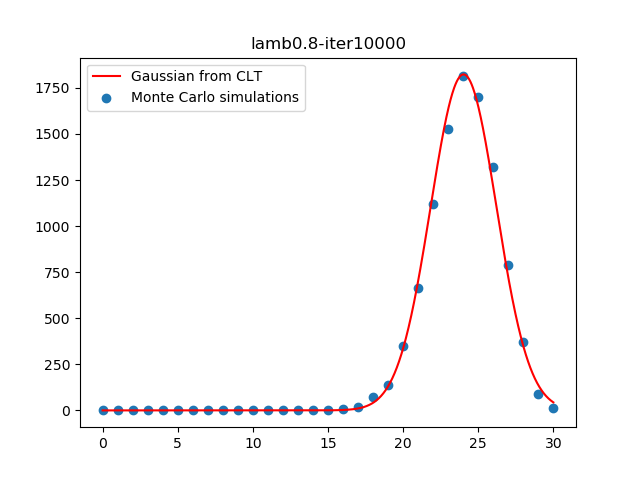
\includegraphics[width=4cm]{5_6_picture/lamb0_8-iter10000.png}
		%\caption{fig2}
		\end{minipage}%
		}%
		\subfigure[$\lambda=0.9$]{
		\begin{minipage}[t]{0.25\linewidth}
		\centering
		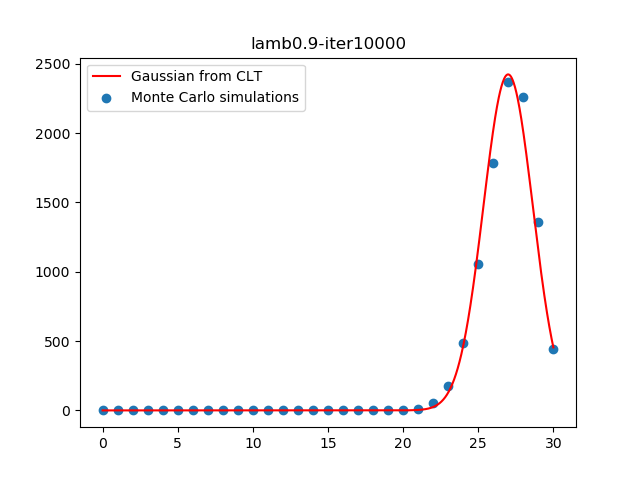
\includegraphics[width=4cm]{5_6_picture/lamb0_9-iter10000.png}
		%\caption{fig2}
		\end{minipage}%
		}%
		
		\centering
		\caption{Monte Carlo simulation and CLT results in 5.6.d}
		\label{pics56}
		\end{figure}
\begin{enumerate}
	\item[(a)] 
		\begin{equation}
		\begin{aligned}
		\notag
		P(X=x) &=l_{n \rightarrow \infty}\left(\begin{array}{l}
		n \\
		x
		\end{array}\right) p^{x}(1-p)^{n-x}  \\
		&=l_{n \rightarrow \infty}\left(\begin{array}{l}
		n \\
		x
		\end{array}\right)\left(\frac{\lambda}{n}\right)^{x}\left(1-\frac{\lambda}{n}\right)^{n-x}  \\
		&=l_{n \rightarrow \infty} \frac{n !}{(n-x) ! x !}\left(\frac{\lambda}{n}\right)^{x}\left(1-\frac{\lambda}{n}\right)^{n}\left(1-\frac{\lambda}{n}\right)^{-x} \\
		&=l_{n=\infty} \frac{n !}{(n-x) !} \frac{1}{n^{x}} \frac{\lambda^{x}}{x !} e^{-\lambda} \quad 1
		\end{aligned}
		\end{equation}
		
		Then, we just need to proof the coefficient of possion is 1.
		\begin{equation}
		\begin{aligned}
		\notag
		&\ell_{h=\infty} \underbrace{\frac{n !}{(n-x) !} \frac{1}{n^{x}}}_{h \rightarrow \infty}=1 . \\
		&\frac{n(n-1)(n-2) \cdots(n-x+1)}{n}=1 .
		\end{aligned}
		\end{equation}
		Thus, 
		\begin{equation} 
		\notag
		\lim _{n \rightarrow \infty} P_{n}(x)=e^{-\lambda} \lambda^{x} /(x !)
		\end{equation}
	\item [(b)]
		According to the definition in section 5.2, central limit theorem is the limiting distribution of $S_{n} / \sqrt{n \sigma^{2}}$ as $n \rightarrow \infty$ is a Gaussian with mean zero and unit variance with $S_{n}=\sum_{t=1}^{n}\left(X_{t}-\mu \right)$. 
		
		But  the conclusion in (a) is not conflict with central limit theorem, since $X_1, \ldots, X_n$ in Exp 5.6 with common mean $p=p_{n}=\lambda / n$ which does not satisfy the assumptions of variable's independence in the central limit theorem.
	\item [(d)] The comparison of Monte Carlo simulation and CLT results can be found in Fig. \ref{pics56}.
		Our observation is that, when $n$ becomes larger and can be regarded as continuous, the poisson distribution is more close to the normal distribution.
\end {enumerate}
\end{proof}




\noindent\textbf{5.7}


(a)If X is $\sigma-$subgaussian , then $E(X)=0$,$E(X^2)\leq\sigma^2$

proof:

\begin{equation}
E(e^{\lambda X}) = \sum_{n=0}^{\infty}\frac{\lambda^n E(X^n)}{n!}=1+\lambda E(X)+\frac{\lambda^2 E(X^2)}{2}+O(\lambda^2)
\end{equation}

By definition ,

\begin{equation}
E(e^{\lambda X})\leq e^{\frac{\lambda^2 \sigma^2}{2}}=1+\frac{\lambda^2 \sigma^2}{2}+O(\lambda^2)
\end{equation}

By comparing the above two formulas and discussing the case that a approaches to 0 from above and below 0, we get the conclusion that ,

$E(X)=0$,$E(X^2)\leq\sigma^2$

(b)

If X is $\sigma-$subgaussian , then $E(X)=0$,$E(X^2)\leq\sigma^2$ .

$E(e^{c\lambda x}) = 1+\lambda E(cx)+\frac{\lambda^2 E(c^2 x^2)}{2}+O(\lambda^2)$

$\leq 1+c\lambda E(x)+\frac{\lambda^2 c^2}{2} E(x^2)+O(\lambda^2)$

$\leq 1+\frac{\lambda^2 c^2 \sigma^2}{2}+O(\lambda^2)$

$\leq e^{\frac{\lambda^2 c^2 \sigma^2}{2}}$

Hence , cX is $|c|\sigma-$subgaussian .

(c)

If $X_1$ is $\sigma_1-$subgaussian , $X_2$ is $\sigma_2-$subgaussian

then $E(X_1)=0$,$E(X_1^2)\leq\sigma_1^2$ ,$E(X_2)=0$,$E(X_2^2)\leq\sigma_2^2$

$E(e^{\lambda (x_1+x_2)}) = 1+\lambda E(x_1+x_2)+\frac{\lambda^2 E((x_1+x_2)^2)}{2}+O(\lambda^2)$

$= 1+\frac{\lambda^2}{2} Var(x_1+x_2)+O(\lambda^2)$

$= 1+\frac{\lambda^2}{2} (var(x_1)+var(x_2)+2cov(x_1,x_2))+O(\lambda^2)$

Because $x_1$, $x_2$ are independent ,

$= 1+\frac{\lambda^2}{2} (E(x_1^2) + E(x_2^2))(\lambda^2)$

$\leq 1+\frac{\lambda^2}{2} (\sigma_1^2 + \sigma_2^2)+O(\lambda^2)$

$\leq e^{\frac{\lambda^2 (\sigma_1^2 + \sigma_2^2)}{2}}$

Hence , $X_1+X_2$ is $\sqrt{\sigma_1^2 + \sigma_2^2}-$subgaussian .



\noindent\textbf{5.8}
(\textsc{Properties of subgaussian random variables (ii)})
Let $X_{i}$ be $\sigma_i$-subgaussian for $i \in\{1,2\}$ with $\sigma_i \geq 0$.
Prove that $X_{1}+X_{2}$ is $(\sigma_1 + \sigma_2)$-subgaussian.
Do \textit{not} assume independence of $X_1$ and $X_2$.

\begin{proof}
	We start straight from the definition:

	\begin{equation*}
	\begin{aligned}
	&\mathbb{E}[\exp(\lambda(X_{1}+X_{2}))]\\
	\leq &\mathbb{E}[\exp(\lambda p X_{1})]^\frac{1}{p} \mathbb{E}[\exp(\lambda q X_{2})]^\frac{1}{q}\\
	\leq &\exp(\lambda^2 p^2 \sigma_1^2 / 2)^\frac{1}{p} \exp(\lambda^2 q^2 \sigma_2^2 / 2)^\frac{1}{q}\\
	= &\exp(\frac{\lambda^2(p \sigma_1^2 + q \sigma_2^2)}{2})\\
	= &\exp(\frac{\lambda^2(\sigma_1^2 + \sigma_2^2)}{2}),
	\end{aligned}
	\end{equation*}
	where the first inequality holds according to Hölder's inequality and the last equality holds with $p = \frac{\sigma_1^2 + \sigma_2^2}{\sigma_2^2}$.
\end{proof}

\noindent\textbf{5.9}
(Properties of moment/cumulative-generating functions) Let $X$ be a real-valued random variable and let $M_X(\lambda) = \EE{\exp(\lambda X)}$ be its moment-generating function defined over $\text{dom}(M_X) \subseteq \RR$, where the expectation takes on finite values. Show that the following properties hold:
\begin{enumerate}
	\item[(a)] $M_X$ is convex, and in particular $\text{dom}(M_X)$ is an interval containing zero.
	\item[(b)] $M_X(\lambda) \ge e^{\lambda \EE{X}}$ for all $\lambda \in \text{dom}(M_X)$.
	\item[(c)] For any $\lambda$ in the interior of $\text{dom}(M_X)$, $M_X$ is infinitely many times differentiable.
	\item[(d)] Let $M^{(k)}_X(\lambda) = \frac{d^k}{d\lambda^k}M_X(\lambda)$. Then, for $\lambda$ in the interior of $\text{dom}(M_X)$, $M^{(k)(\lambda)} = \EE{X^k \exp(\lambda X)}$. 
	\item[(e)] Assuming $0$ is in the interior of $\text{dom}(M_X)$, $M^{(k)(0)} = \EE{X^k}$ (hence the name of $M_X$).
	\item[(f)] $\psi_X$ is convex (that is, $M_X$ is log-convex). 
\end{enumerate}

\begin{proof}

\begin{enumerate}
	\item[(a)] To prove $M_X$ is convex, we want to prove $\forall \alpha \in (0,1), a,b\in \text{dom}(M_X)$, there is $M_X(\alpha 
	 a + (1-\alpha)b) \le \alpha M_X(a) + (1-\alpha)M_X(b)$. 
	 \begin{align*}
	 	M_X(\alpha a + (1-\alpha)b) &= \EE{ \exp\bracket{ \alpha a + (1-\alpha)b X }} \\
	 	&\le \EE{ \alpha \exp\bracket{ a X}+ (1-\alpha)\exp\bracket{b X} } \\
	 	&= \alpha \EE{\exp\bracket{ a X}}+(1-\alpha)\EE{\exp\bracket{b X}} = \alpha M_X(a) + (1-\alpha)M_X(b)\,,
	 \end{align*}
	 where the inequality comes from the convexity of $x \to \exp(x)$.

	 To prove $\text{dom}(M_X)$ is an interval containing zero, we want to prove $M_X(0)<\infty$. It is obvious that $ M_X(0) = \EE{\exp(0\cdot X)} = \EE{\exp(0)} =1<\infty $. 
	\item[(b)] For all $\lambda \in \text{dom}M_X$, we have
	\begin{align*}
		M_X(\lambda) = \EE{ \exp(\lambda X) } \ge \exp\bracket{\EE{\lambda X}} = \exp\bracket{\lambda\EE{ X}}\,,
	\end{align*}
	where the inequality comes from the convexity of $x \to \exp(x)$.
	\item[(c)] TBD
	\item[(d)] $M^{(1)}_X(\lambda) = \frac{d}{d\lambda} \EE{\exp(\lambda X)}= \EE{\frac{d}{d\lambda} \exp(\lambda X)} = \EE{X \exp(\lambda X)}$. 
	Recursively, we have $M^{(k)}_X(\lambda) = \EE{X^k \exp(\lambda X)}$. 
	\item[(e)] According to the result of (d), we have $M^{(k)}_X(0) = \EE{X^k \exp(0\cdot X)} = \EE{X^k}$.
	\item[(f)] To prove $\psi_X$ is convex, we want to prove $\forall \alpha \in (0,1), a,b\in \text{dom}(\psi_X)$, there is $\psi_X(\alpha a + (1-\alpha)b) \le \alpha \psi_X(a) + (1-\alpha)\psi_X(b)$.
	\begin{align*}
		\psi_X(\alpha a + (1-\alpha)b) &= \log M_X( \alpha a + (1-\alpha)b ) \\
		&= \log \EE{\exp\bracket{ \alpha a + (1-\alpha)b}X} \\
		&= \log \EE{\exp\bracket{ \alpha aX } \exp((1-\alpha)bX)} \\
		&= \log \EE{\bracket{\exp\bracket{ aX }}^{\alpha} \bracket{\exp(bX)}^{(1-\alpha)}}\\
		&\le  \log \bracket{ \EE{\exp\bracket{ aX }}^{\alpha } \EE{\exp(bX)}^{(1-\alpha)} } \\
		&= \alpha \log \EE{ \exp\bracket{ aX } } + (1-\alpha) \EE{\exp(bX)} = \alpha \psi_X(a) + (1-\alpha)\psi_X(b) \,,
	\end{align*}
	where the inequality comes from the Hölder's inequality. 
\end{enumerate}

\end{proof}


\noindent\textbf{5.10} (Large deviation theory) Let $X,X_1,X_2,...,X_n$ be a sequence of independent and identically distributed random variables with zero mean and moment-generating function $M_X$ with $dom(M_X)=\RR.$ Let$\hat{\mu}_n=\frac{1}{n}\sum_{t=1}^nX_t$.
\begin{enumerate}
    \item[(a)]Show that for any $\epsilon>0$,
        \begin{align}
            \frac{1}{n}\log\PP{\hat{\mu}_n\geq\epsilon}\leq -\psi_X^{\ast}(\epsilon)=-\underset{\lambda}{\sup}(\lambda\epsilon-\log M_X(\lambda))
        \end{align}
    \item[(b)]Show that when X is a Rademacher variable$(\PP{X=1}=\PP{X=-1}=\frac{1}{2})$,$\psi_X^{\ast}(\epsilon)=\frac{1+\epsilon}{2}\log(1+\epsilon)+\frac{1-\epsilon}{2}\log(1-\epsilon)$when$\abs{\epsilon}\le 1$ and $\psi_X^{\ast}(\epsilon)=+\infty$,otherwise.
\end{enumerate}

\begin{proof}
\begin{enumerate}
	\item[(a)] For all $\lambda\in domM_X$,we have 
	    \begin{align*}
	        \frac{1}{n}\log\PP{\hat{\mu}_n\geq\epsilon}&=\frac{1}{n}\log\PP{\exp{(\lambda n\hat{\mu}_n)}\geq\exp{(\lambda n \epsilon)}}\\
	        &\leq \frac{1}{n}\log(\EE{\exp{(\lambda n\hat{\mu}_n)}}\exp{(-\lambda n \epsilon)})\\
	        &=\frac{1}{n}\log(\prod_{t=1}^n\EE{\exp{(\lambda X_t)}}\exp{(-\lambda n \epsilon)})\\
	        &=\frac{1}{n}\log(\EE{\exp{(\lambda X)}}^n\exp{(-\lambda n \epsilon)})\\
	        &=\log(\EE{\exp{(\lambda X)}}\exp{(-\lambda\epsilon)})\\
	        &=-(\lambda\epsilon-\log M_X(\lambda))
	    \end{align*}
        Since it holds for all $\lambda\in domM_X$,we can imply
        \begin{align*}
            \frac{1}{n}\log\PP{\hat{\mu}_n\geq\epsilon}\leq -\psi_X^{\ast}(\epsilon)=-\underset{\lambda}{\sup}(\lambda\epsilon-\log M_X(\lambda))
        \end{align*}

	\item[(b)] By definition, $\psi_{X}(\lambda)=\log(\frac{1}{2}(\exp (-\lambda)+\exp (\lambda)))= \log(\cosh (\lambda))$, where $\cosh(\cdot)$ is the hyperbolic cosine function.
	To find the maximum of $f(\lambda) = \lambda \varepsilon - \psi_{X}(\lambda)$, we have $f^\prime(\lambda) = \varepsilon - \tanh(\lambda)$, where $\tanh(\lambda) = \frac{\exp(\lambda) - \exp(-\lambda)}{\exp(\lambda) + \exp(-\lambda)}$ is the hyperbolic tangent function.
	Since $\tanh(\lambda) \in[-1,1]$, $\sup _{\lambda} f(\lambda)=+\infty$ when $|\varepsilon|>1$.
	Otherwise, we have
	\begin{equation*}
		\begin{aligned}
			\psi_{X}^{*}(\varepsilon)
			&=f\left(\tanh ^{-1}(\varepsilon)\right)\\
			&=\tanh ^{-1}(\varepsilon) \varepsilon-\log \cosh \left(\tanh ^{-1}(\varepsilon)\right)\\
			&=\frac{\varepsilon}{2} \log \left(\frac{1+\varepsilon}{1-\varepsilon}\right)+\frac{1}{2} \log \left(1-\varepsilon^{2}\right)\\
			&=\frac{1+\varepsilon}{2} \log (1+\varepsilon)+\frac{1-\varepsilon}{2} \log (1-\varepsilon),
		\end{aligned}
	\end{equation*}
	where the second equality holds as $\tanh ^{-1}(\varepsilon)=\frac{1}{2} \log \left(\frac{1+\varepsilon}{1-\varepsilon}\right)$.
\end{enumerate}
\end{proof}


\noindent\textbf{5.11} (Hoeffding's lemma) Suppose that $X$ is zero mean and $X \in [a,b]$ almost surely for constants $a <b$.
\begin{enumerate}
	\item[(a)]Show that $X$ is $(b-a)/2$-subgaussian.
	\item[(b)]Prove Hoeffding's inequality (Lemma \ref{lem:hoeffding}).
\end{enumerate}
\begin{lemma}[Hoeffding's inequality]\label{lem:hoeffding}
	For a zero-mean random variable $X$ such that $X \in [a,b]$ almost surely for real values $a <b$, then $M_X(\lambda) \le \exp(\lambda^2 (b-a)^2 / 8)$. Applying the Cramér–Chernoff method shows that if $X_1,X_2,\ldots,X_n$ are independent and $X_t \in [a_t,b_t]$ almost surely with $a_t < b_t$ for all $t$. Then, 
	\begin{align}
		\PP{\frac{1}{n} \sum_{t=1}^n \bracket{X_t - \EE{X_t}} \ge \varepsilon } \le \exp\bracket{ \frac{-2n^2\varepsilon^2}{\sum_{t=1}^n (b_t-a_t)^2 } }\,.
	\end{align}
\end{lemma}

\begin{proof}
\begin{enumerate}
	\item[(a)]To show $X$ is $(b-a)/2$-subgaussian, we want to prove $\forall \lambda \in \RR, \EE{\exp(\lambda X)} \le \exp\bracket{ \frac{\lambda^2 (b-a^2)}{8} }$.

	According to the convexity of $x \to \exp(x)$ and Jensen's inequality, we have $\forall X \in [a,b]$,
	\begin{align*}
		\exp(\lambda X) = \exp\bracket{ \frac{b-X}{b-a}\lambda a + \frac{X-a}{b-a}\lambda b } \le \frac{b-X}{b-a}\exp(\lambda a)+ \frac{X-a}{b-a}\exp(\lambda b)\,.
	\end{align*}
	Thus, 
	\begin{align*}
		\EE{\exp(\lambda X)} &\le \frac{b-\EE{X}}{b-a}\exp(\lambda a)+ \frac{\EE{X}-a}{b-a}\exp(\lambda b) \\
		&= \frac{b}{b-a}\exp(\lambda a)+ \frac{-a}{b-a}\exp(\lambda b)\\
		&= (1-\theta)\exp(\lambda a)+\theta \exp(\lambda b) ~~~\bracket{\text{By letting $\theta = \frac{-a}{b-a}$}} \\
		&= \exp(\lambda a) \bracket{1-\theta+\theta \exp(\lambda b - \lambda a)} \\
		&= \exp(-\lambda(b-a)\theta) \bracket{ 1-\theta+\theta \exp(\lambda b - \lambda a) } ~~~\bracket{\text{By representing $a$ using $\theta$}}\\
		&= \exp\bracket{-\theta u + \log(1-\theta+\theta\exp(u))} ~~~\bracket{\text{By letting $u=\lambda(b-a)$} } \\
		&= \exp(\phi(u)), ~~~\text{where}~~ \phi(u)=-\theta u + \log(1-\theta+\theta\exp(u))\,.
	\end{align*}
	We next want to find the upper bound for $\exp(\phi(u))$. According to the Taylor's theorem with mean-values forms of the remainder, we have 
	\begin{align*}
		\phi(u) &= \phi(0) + u\phi'(0) + \frac{1}{2}u^2 \phi''(v),~~~~\text{where}~v \in (0,u)\\
		&= \frac{1}{2}u^2 \phi''(v) ~~~\bracket{\text{Since $\phi(0) = \phi'(0) = 0$}}\\
		&= \frac{1}{2}u^2 \cdot \frac{\theta \exp(v)}{1-\theta+\theta \exp(v)}\bracket{1-\frac{\theta \exp(v)}{1-\theta+\theta \exp(v)}} \\
		&\le \frac{1}{2}u^2 \cdot \frac{1}{4} =\frac{1}{8}u^2 = \frac{\lambda^2 (b-a)^2}{8}\,.
	\end{align*}
	Above all, we have proved that $\forall \lambda \in \RR, \EE{\exp(\lambda X)} \le \exp(\phi(u)) \le \exp\bracket{\frac{\lambda^2 (b-a)^2}{8}}$. 


	\item[(b)]  We only give the upper tail of the Hoeffding's Inequality using the Hoeffding's Lemma since the lower tail has a similar proof. Applying the Hoeffding' Lemma and the Chernoff bound technique immediately
	shows that
	\begin{align*}
		\mathbb{P}\left(\frac{1}{n}\sum^n_{t=1}(X_t -\mathbb{E}[X_t])\geq\epsilon\right)&=\mathbb{P}\left(\sum^n_{t=1}(X_t-\mathbb{E}[X_t])\geq n\epsilon \right)\\
		&\leq\mathbb{E}\left[\exp\left(\lambda\sum^n_{t=1}(X_t-\mathbb{E}[X_t]) \right) \right]e^{-\lambda n\epsilon}\\
		&=\left(\Pi^n_{t=1}\mathbb{E}[\exp\left(\lambda(X_t-\mathbb{E}[X_t])\right)] \right)e^{-\lambda n\epsilon}\\
		&\leq\left(\Pi^n_{t=1}e^{\frac{\lambda^2(b_t-a_t)^2}{8}} \right)e^{-\lambda n\epsilon}\,,
	\end{align*}
	where $\lambda\geq0$. Minimizing the RHS of the above inequality over $\lambda$ shows that
	\begin{align*}
		\mathbb{P}\left(\frac{1}{n}\sum^n_{t=1}(X_t -\mathbb{E}[X_t])\geq\epsilon\right)\leq \min_{\lambda\geq0}\left(\Pi^n_{t=1}e^{\frac{\lambda^2(b_t-a_t)^2}{8}} \right)e^{-\lambda n\epsilon} =\exp\left(\frac{-2n^2\epsilon^2}{\sum^n_{t=1}(b_t-a_t)^2}\right)\,.
	\end{align*}
\end{enumerate}
\end{proof}


\noindent \textbf{5.14}(Bernstein’s inequality) Let $X_1,X_2,\ldots,X_n$ be a sequence of independent random variables with $X_t - \EE{X_t} \le b$ almost surely and $S= \sum_{t=1}^n X_t -\EE{X_t}$ and $v = \sum_{t=1}^n \mathbb{V}[X_t]$.
\begin{enumerate}
	\item[(a)] Show that $g(x) = \frac{1}{2} + \frac{x}{3!}+\frac{x^2}{4!}+\cdots = \frac{\exp (x) - 1 -x}{x^2}$ is increasing.
	\item[(b)] Let $X$ be a random variable with $\EE{X}=0$ and $X\le b$ almost surely. Show that $\EE{\exp (X)} \le 1+g(b)\mathbb{V}[X]$.
	\item[(c)] Prove that $(1+\alpha)\log(1+\alpha) - \alpha \ge \frac{3\alpha^2}{6+2\alpha}$ for all $\alpha\ge 0$. Prove that this is the best possible approximation in the sense that the $2$ in the denominator cannot be increased.
	\item[(d)] Let $\varepsilon > 0$ and $\alpha = b\varepsilon/v$ and prove that
	\begin{align}
		\PP{S\ge \varepsilon} &\le \exp\bracket{ -\frac{v}{b^2}\bracket{ (1+\alpha)\log(1+\alpha) -\alpha} } \label{eq:5-14-d-1}\\
		&\le \exp\bracket{- \frac{\varepsilon^2}{2v\bracket{ 1+\frac{b\varepsilon}{3v} }} } \label{eq:5-14-d-2}\,.
	\end{align}
	\item[(e)] Use the previous result to show that
	\begin{align*}
		\PP{S\ge \sqrt{2v \log\bracket{\frac{1}{\delta}}}+ \frac{2b}{3}\log\bracket{\frac{1}{\delta}}}  &\le \delta \,.
	\end{align*}
	\item[(f)] Let $X_1,X_2,\ldots,X_n$ be a sequence of random variables adapted to filtration $\mathbb{F} = (\cF_t)_t$. Abbreviate $\mathbb{E}_t[\cdot] = \EE{\cdot \mid \cF_t}$ and $\mu_t = \mathbb{E}_{t-1}[X_t]$. Define $S = \sum_{t=1}^n X_t - \mu_t$ and let $V = \sum_{t=1}^n \mathbb{E}_{t-1}[(X_t - \mu_t)^2]$ be the predictable variation of $\bracket{\sum_{t=1}^p X_t-\mu_t }_p$. Show that if $X_t - \mu_t \le b$ holds almost surely for all $t \in [n]$, then with $\alpha = b\varepsilon / v$, 
	\begin{align*}
		\PP{S\ge \varepsilon,V\le v} \le \exp\bracket{ -\frac{v}{b^2}\bracket{ (1+\alpha)\log (1+\alpha)-\alpha } } \,.
	\end{align*}
	Note that the right-hand side of this inequality is the same as that shown in Eq.\eqref{eq:5-14-d-1}.
\end{enumerate}

\begin{proof}
	\begin{enumerate}
		\item[(a)] To show $g(x)$ is increasing, we want to show that $g'(x)\ge 0$. 
		\begin{align*}
			g'(x) &= \frac{(\exp(x)-1)x^2 - (\exp(x)-x-1)2x}{x^4} \\
			&= \frac{x(x-2)\exp(x)+x(x+2)}{x^4}\,.
		\end{align*}
		By letting $g'(x)=0$, we find $x=0$. And $\forall x\neq 0$, we have $g'(x)>0$. Above all, we can show $g(x)$ is increasing. 
		\item[(b)] According to (a), we have $\exp(x) = x^2 g(x)+x+1$. Thus 
		\begin{align*}
			\EE{\exp(X)} = \EE{ X^2 g(X)+X+1 } &= \EE{X^2 g(X)}+\EE{X}+1\\
			&\le g(b)\EE{X^2}+\EE{X}+1\\
			&= g(b) \bracket{\mathbb{V}[X]+\EE{X}^2}+\EE{X}+1 \\
			&= g(b)\mathbb{V}[X]+1\,,
		\end{align*}
		where the inequality is because $X\le b$ and the increasing property of $g(x)$ proved in (a), the second last equality comes from the definition of $\mathbb{V}[X]$, the last equality holds since $\EE{X}=0$.
		\item[(c)]
		\item[(d)] 
		\item[(e)] 
		By choosing $\delta = \exp\bracket{ -\frac{\varepsilon^2}{2v\bracket{1+\frac{b\varepsilon}{3v}}} }$, we have
		\begin{align*}
			\varepsilon^2 - 2v\log\bracket{\frac{1}{\delta}} - \frac{2b}{3}\varepsilon\log\bracket{\frac{1}{\delta}} = 0\,.
		\end{align*}
		By solving this equality, we have 
		\begin{align*}
			\varepsilon = \frac{1}{2}\sqrt{ \bracket{\frac{2b}{3}\log \bracket{\frac{1}{\delta}}}^2 + 8v\log \bracket{\frac{1}{\delta}}}+\frac{b}{3}\log \bracket{\frac{1}{\delta}}
		\end{align*}
		Then according to Eq.\eqref{eq:5-14-d-2}, 
		\begin{align*}
		\PP{S \ge \sqrt{2v\log \bracket{\frac{1}{\delta}}}+\frac{2b}{3}\log \bracket{\frac{1}{\delta}}} &= \PP{S \ge \sqrt{2v\log \bracket{\frac{1}{\delta}}}+\frac{b}{3}\log \bracket{\frac{1}{\delta}}+\frac{b}{3}\log \bracket{\frac{1}{\delta}}}\\
			&\le
			\PP{S \ge \frac{1}{2}\sqrt{ \bracket{\frac{2b}{3}\log \bracket{\frac{1}{\delta}}}^2 + 8v\log \bracket{\frac{1}{\delta}}}+\frac{b}{3}\log \bracket{\frac{1}{\delta}}} \le \delta \,,
		\end{align*}
		where the first inequality is because $\forall a,b\in \RR: \sqrt{|a|+|b|} \le \sqrt{|a|}+\sqrt{|b|}$




	\end{enumerate}
\end{proof}





\noindent \textbf{5.16}
By assumption $Pr(X_t\leq x)\leq x$, which means that for$\lambda <1$,
\begin{align}
\mathbb{E}\left[exp(\lambda log(\frac{1}{x_t}))\right] = \int_0^\infty P(exp(\lambda log(\frac{1}{x_t}))\geq x)dx = 1 +\int_1^\infty P(X_t \leq x^{-\frac{1}{\lambda}})dx
\end{align}
Applying the Cramer-Chernoff method,
$$P\left(\sum_{t=1}^n log(\frac{1}{X_t}) \geq \epsilon\right) = P\left(exp(\lambda \sum_{t=1}^n log(\frac{1}{X_t})) \geq exp(\lambda \epsilon) \right) \leq \left(\frac{1}{1-\lambda}\right)^n exp (-\lambda \epsilon)$$
choosing $\lambda  = \frac{\epsilon-n}{\epsilon}$ completes the claim.







\noindent \textbf{5.18} (\textsc{Expectation of maximum})
Let $X_{1}, \ldots, X_{n}$ be a sequence of $\sigma$-subgaussian random variables
(possibly dependent) and $Z=\max _{t \in[n]} X_{t}$. Prove that

\begin{itemize}
	\item[(a)] $\mathbb{E}[Z] \leq \sqrt{2 \sigma^{2} \log (n)}$.
	\item[(b)] $\mathbb{P}\left(Z \geq \sqrt{2 \sigma^{2} \log (n / \delta)}\right) \leq \delta \text { for any } \delta \in(0,1)$.
\end{itemize}

\begin{proof}
	\begin{itemize}
		\item[(a)] Let $\lambda >0$.
		Then,
		\begin{equation*}
			\exp(\lambda \mathbb{E}[Z]) \leq \mathbb{E}[\exp(\lambda Z)] \leq \sum_{t=1}^n \mathbb{E}[\exp(\lambda X_t)] \leq n \exp(\frac{\lambda^2 \sigma^2}{2}).
		\end{equation*}
		
		Rearranging shows that
		\begin{equation*}
			\mathbb{E}(Z) \leq \frac{log(n)}{\lambda} + \frac{\lambda \sigma^2}{2}.
		\end{equation*}
	
		Choosing $\lambda = \frac{1}{\sigma} \sqrt{2log(n)}$ shows that $\mathbb{E}(Z) \leq \sqrt{2\sigma^2 log(n)}$
		
		\item[(b)] First notice that
		\begin{equation*}
			\begin{aligned}
				\mathbb{P}\left(Z \geq \sqrt{2 \sigma^{2} \log (n / \delta)}\right)
				&= \mathbb{P}\left(\exists i: X_i \geq \sqrt{2 \sigma^{2} \log (n / \delta)}\right)\\
				&\leq \sum_{i=1}^n \mathbb{P}\left(X_i \geq \sqrt{2 \sigma^{2} \log (n / \delta)}\right),
			\end{aligned}
		\end{equation*} 
		which is given directly by a union bound.

		Then, according to Theorem 5.3, we have $\mathbb{P}\left(X_i \geq \sqrt{2 \sigma^{2} \log (n / \delta)}\right)
		\leq \frac{\delta}{n}$ to complete the proof.
	\end{itemize}
\end{proof}
